% 本章节是介绍 RISC-V的
\section{计算机组成与设计——基于RISC-V}
本章节是根据 David A. Patterson 的著作\cite{Computer_Organization_and_Design_riscv}以及浙江大学刘鹏博导的公开课\cite{Computer_Organization_and_Design_ZJU}来改编实现的。

\subsection{指令表示方法与指令格式}
如果把计算机比作一个在说话的人,那么指令就是每一个单词,指令集就是全部词汇所构成的词汇表

\subsubsection{R指令}
\textbf{R指令}是用于寄存器与寄存器之间算数运算的

一条R型指令的格式划分如图\ref{fig:R-Format_Instruction_Layout}所示,R型指令可以划分为6个域,其中31-25这7bit宽的是功能码7,24-20这5为是源寄存器2,19-15这5为是源寄存器1,14-12这3bit宽的是功能码3,11-7这5bit宽的目的寄存器rd,6-0这7位宽的操作码(部分规定了该指令是什么指令)。

\begin{figure}[htbp]
  \centering %居中显示
  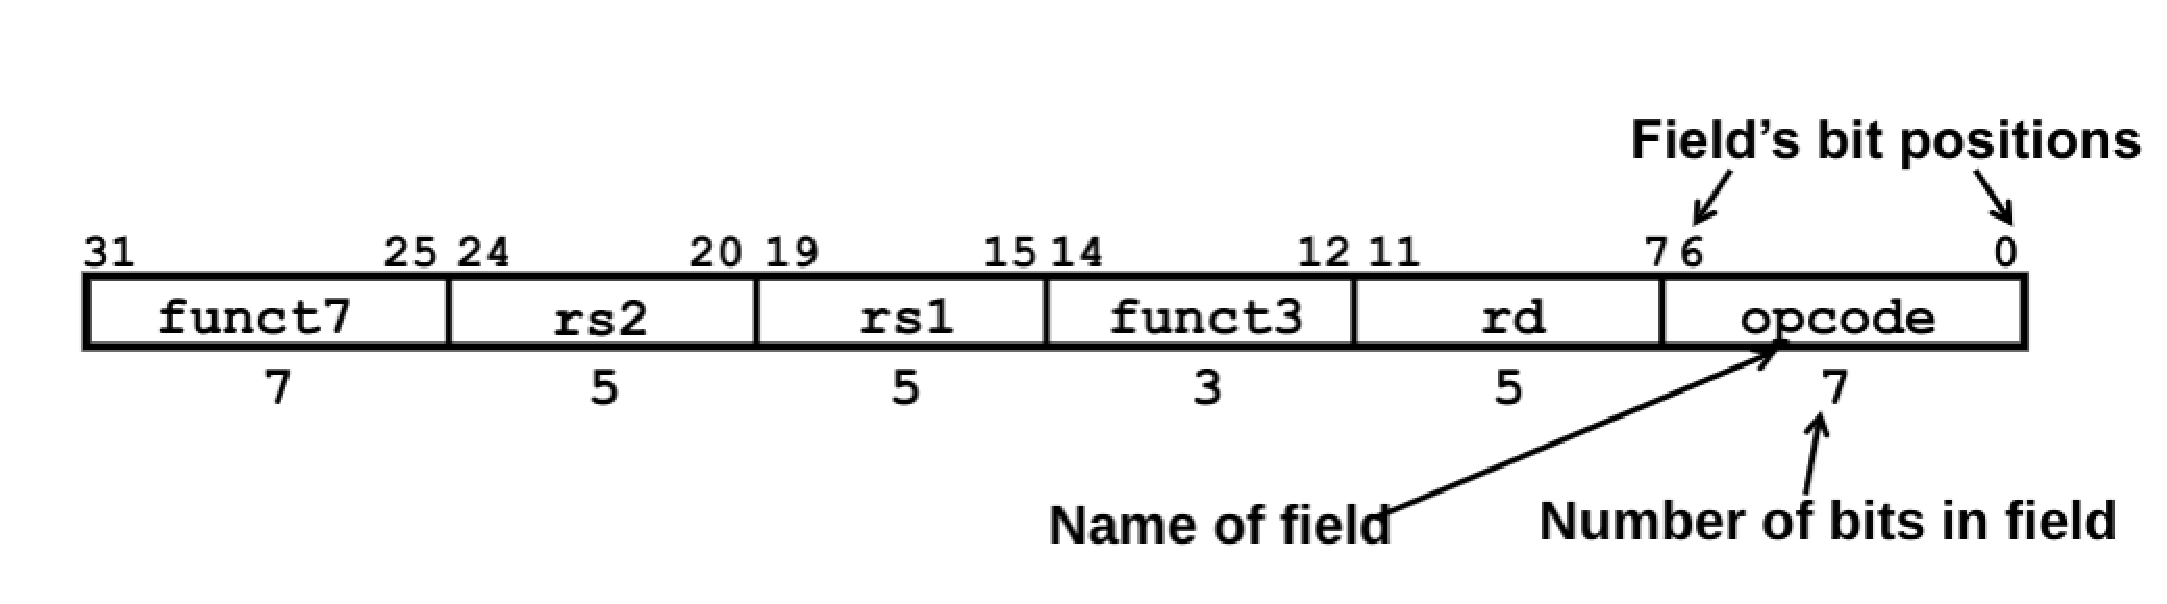
\includegraphics[width=0.8 \textwidth]{figs/RISC-V/指令表示/R-Format_Instruction_Layout.eps}
  \caption{R型指令格式的划分\\ 其中每个域中的文字表示该域的名称;域上的数字表示,该域的起始与终止位置;每个域下面的数字,表示每个域所占据的bit位数}
  \label{fig:R-Format_Instruction_Layout} %设置图形引用名称
\end{figure}
所有R指令的opcode部分都是2进制数:0110011,funct7与funct3是和opcode结合起来一起使用的,三者组合一起规定指令的操作。

rs1,rs2是源寄存器(Source Rggister),用于存放操作数的源地址的,rd是目的寄存器(Destination Rggister),指定接收结果值的寄存器编号,这三个寄存器都存放5位无符号整数(对应十进制$2^5=32$),对应0˜31的通用寄存器中的其中一个。


\subsubsection{I指令}
\textbf{I指令}是用于寄存器与立即数之间算数运算和读取的 

其实如果是我自己设计指令架构,我很有可能将操作寄存器,操作数用一个指令全部实现,但是有一个问题,就是指令中的位长,比方说R指令的源地址和目的地址才5bit,最多就能表示10进制的32位,那要是操作数字就显得有些有限;但是如果你把指令中的位长加长的话,就会造成可以表示的10进制数太多,但是寄存器就32了,造成不必要的浪费。

所以,I型指令可以在R型指令的基础上做一些稍微的改动即可,如图\ref{fig:R_I}所示。

\begin{figure}[htbp]
  \centering %居中显示
  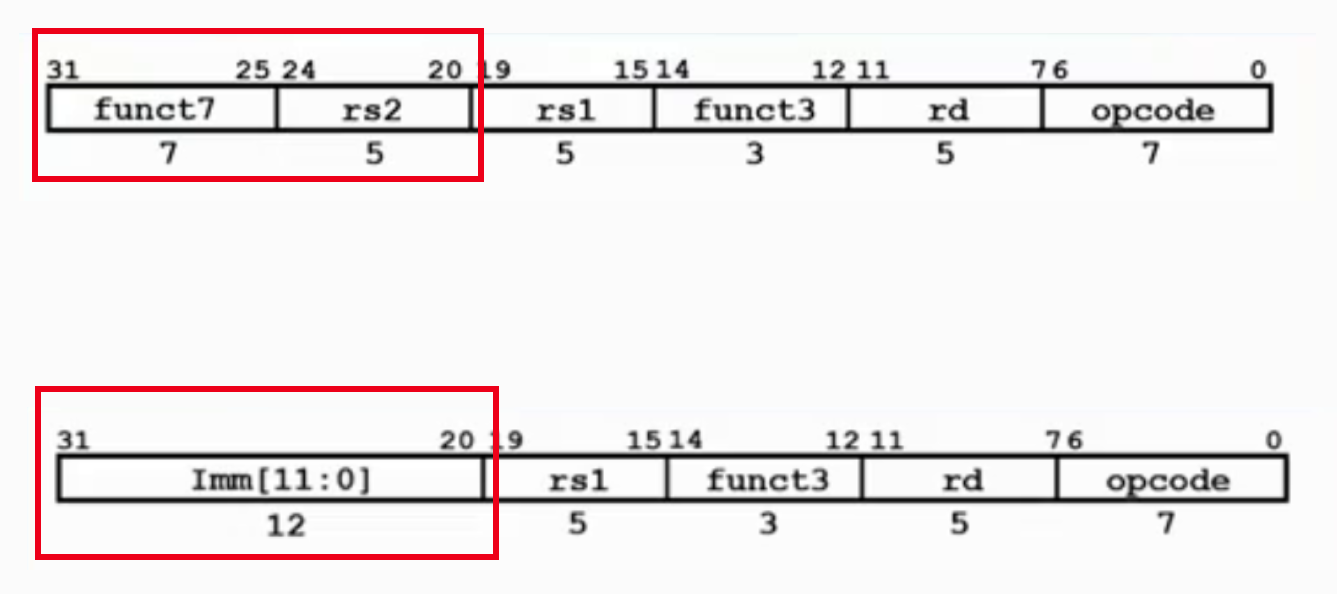
\includegraphics[width=0.8 \textwidth]{figs/RISC-V/指令表示/R_I.eps}
  \caption{I型指令就是把R型指令的前两个域合并成一个了12位的有符号数}
  \label{fig:R_I} %设置图形引用名称
\end{figure}



\subsubsection{S指令}
用于写存储器的

\subsubsection{B指令}
用于分支转移操作的,其实是S指令的一个变体,之前也叫\textbf{SB指令}

\subsubsection{U指令}
用于高20-bit位立即数操作

\subsubsection{J指令}
用于跳转操作,其实是U指令的一个变体,之前也叫\textbf{UJ指令}


\subsection{流水线}
\subsubsection{处理器性能度量方法}
首先,我认为在我们研究之前应该明确我们常说的提高性能是指什么,是表示更快的响应时间?从而更快的完成需要执行的任务?还是单位时间内能完成更多的任务?还是使用寿命更长一些?

我觉得性能的本质是——

\begin{equation}\label{eq:Computer_Analogy}
    \frac{ Time }{ Program } = \frac{ Instructions }{ Program } * \frac{ Cycles }{ Instruction } * \frac{ Time }{ Cycle }
\end{equation}

公式 (\ref{eq:Computer_Analogy})是与处理器性能有关的定理

\subsubsection{流水线的设计}
处理器执行一条指令的步骤——取指,译码,执行,访存,写回。

\subsubsection{结构冒险}
造成这个冒险的原因是硬件不支持同一周期执行多条指令

这个也比较好解决1.让其他阻塞一下等待硬件空闲下来在使用,2.要么就是多添加点硬件。



\subsubsection{数据冒险}
导致数据冒险发生简言之就是不同指令之间存在数据的关联,造成了无法提供指令执行所需的数据,进而指令不能在预期的时钟周期内执行。

解决方案就是 1.让其他阻塞一下等待数据使用完在使用,2.增加一个\textbf{旁路(bypassing)},这样的好处就是不需要等待指令完成就可以超市解决数据冒险。如图\ref{fig:Data_Hazards1} 所示,第一条add指令执行EX阶段的输出前递到sub指令的EX阶段的输入,替换sub指令在第二阶段督促的寄存器X1的值。

\begin{figure}[htbp]
  \centering %居中显示
  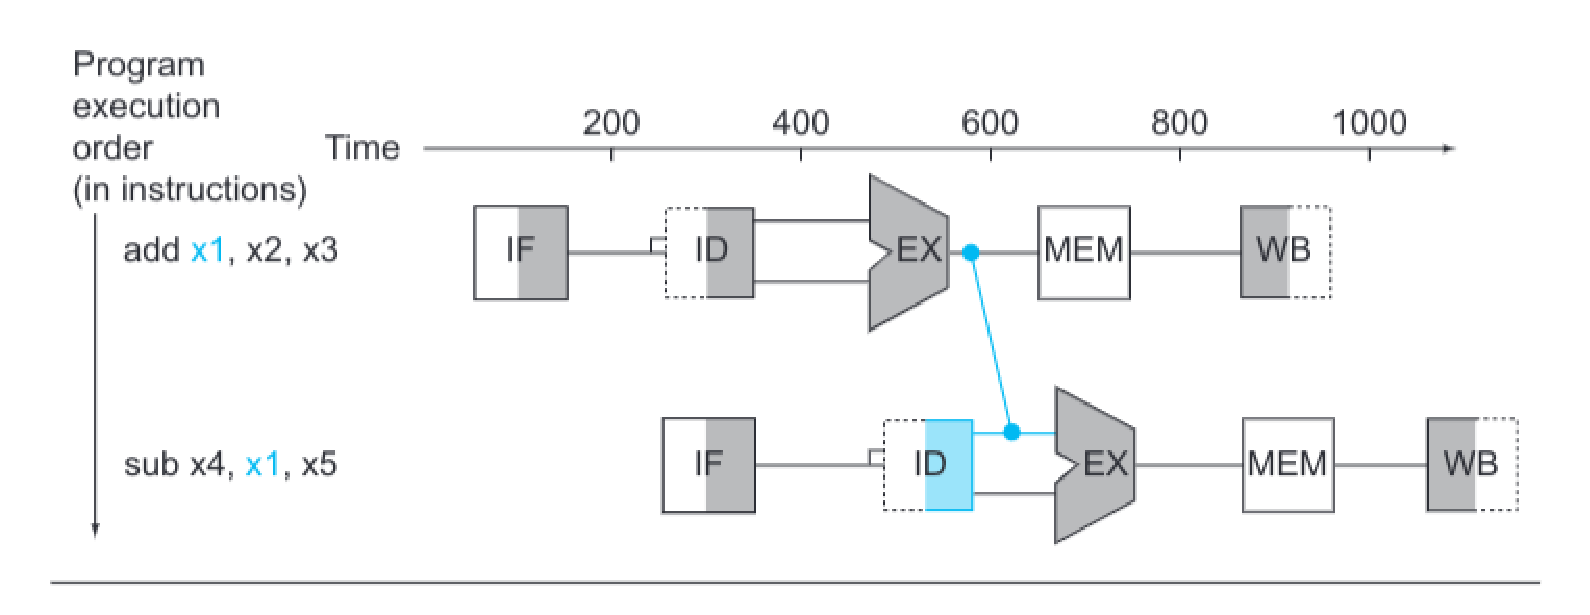
\includegraphics[width=0.8 \textwidth]{figs/RISC-V/流水线/数据冒险1.eps}
  \caption{这张图片就显示了旁路的效果}
  \label{fig:Data_Hazards1} %设置图形引用名称
\end{figure}

但是有时尽管使用了旁路,也不可避免的需要\textbf{流水线停顿(pipeline Stall)},俗称\textbf{气泡(bubble)},图\ref{fig:Data_Hazards2}就是load指令执行之后,紧跟着一条需要使用他结果的R型指令

\begin{figure}[htbp]
  \centering %居中显示
  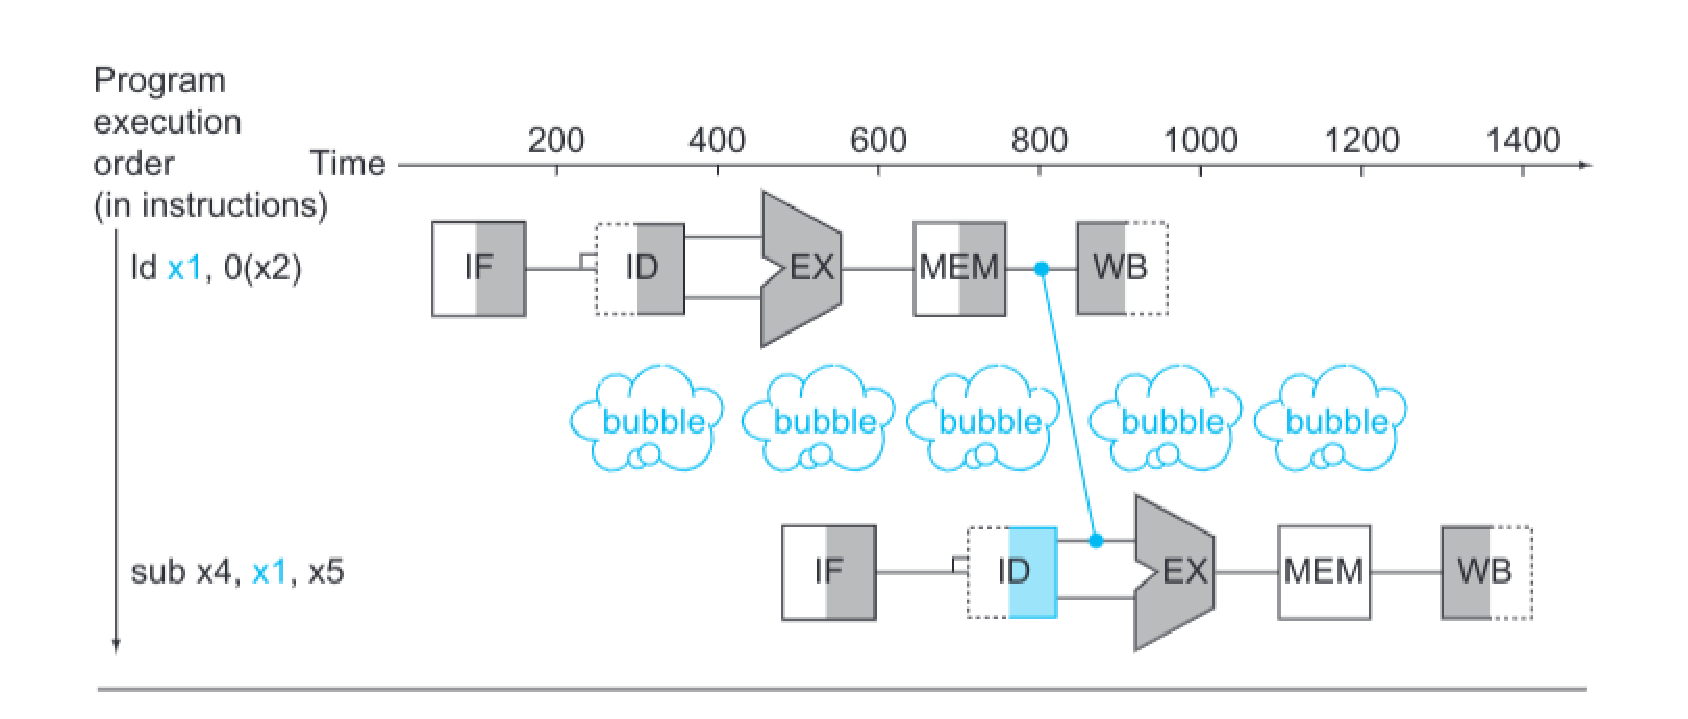
\includegraphics[width=0.8 \textwidth]{figs/RISC-V/流水线/数据冒险2.eps}
  \caption{这张就表示有时即使使用旁路,也许要阻塞等待}
  \label{fig:Data_Hazards2} %设置图形引用名称
\end{figure}


\subsubsection{控制冒险}
这种冒险发生在根据一条指令的结果判断接下来要执行的分支程序。如图\ref{fig:Control_Hazards}所示

\begin{figure}[htbp]
  \centering %居中显示
  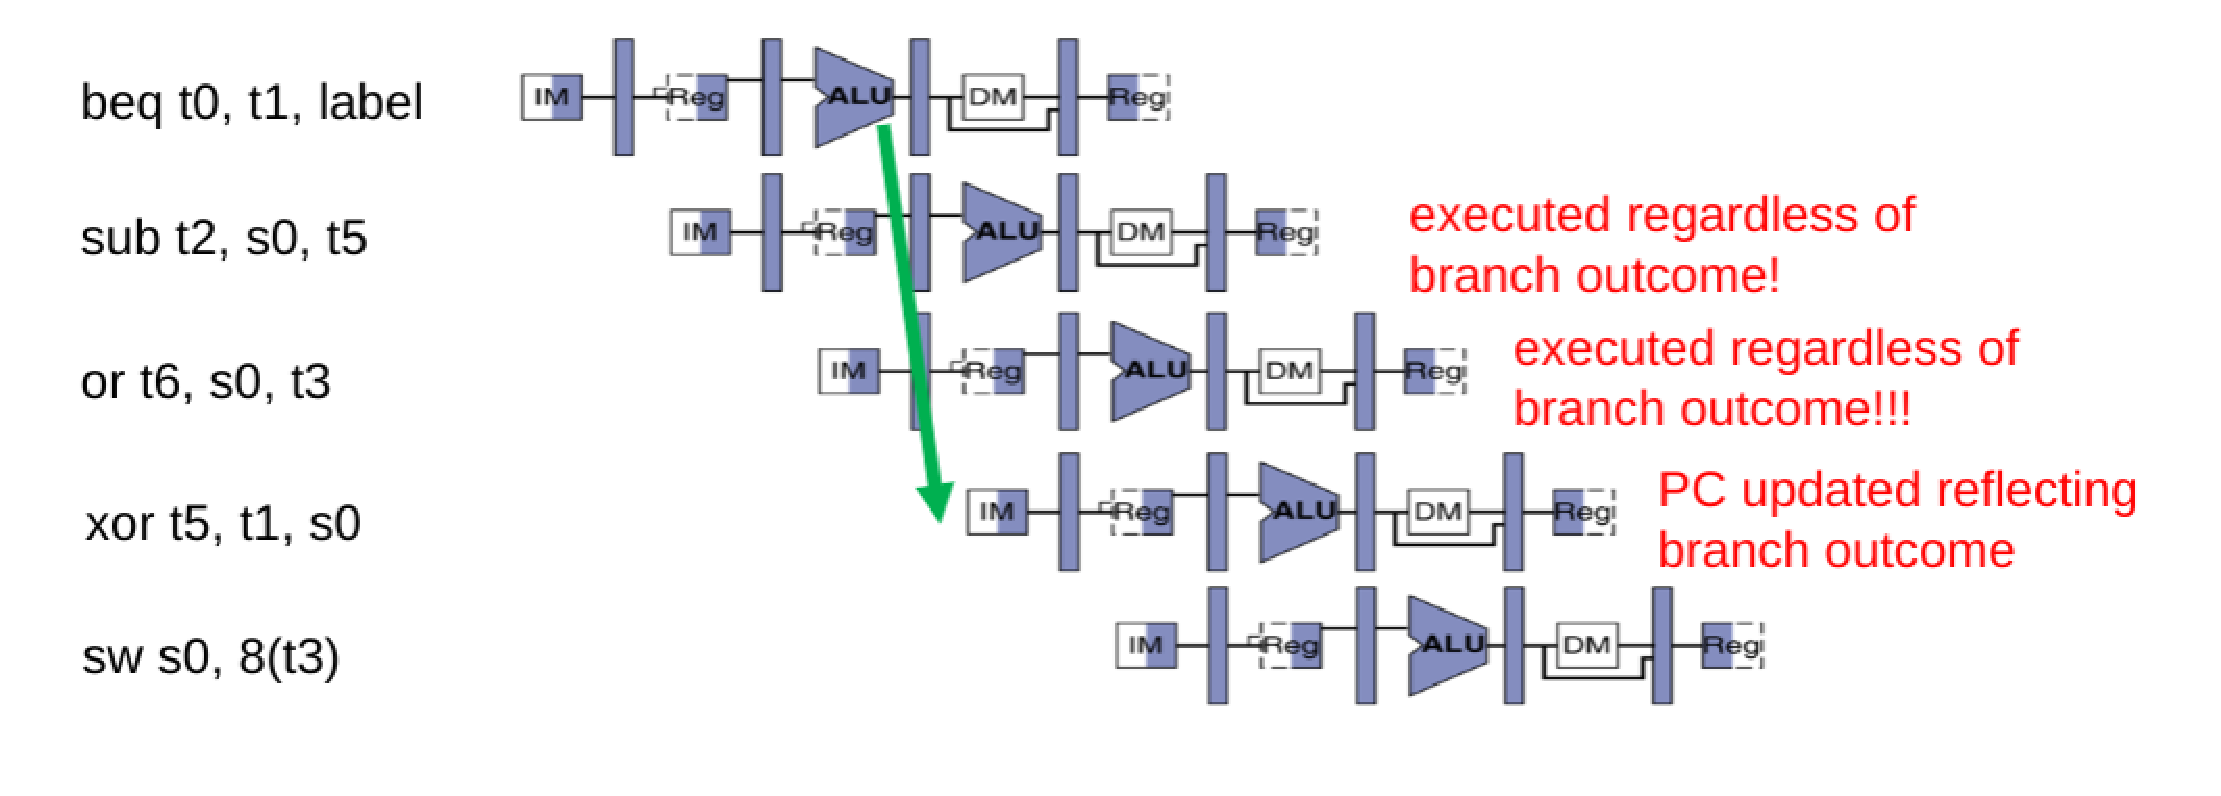
\includegraphics[width=0.8 \textwidth]{figs/RISC-V/流水线/控制冒险.eps}
  \caption{控制冒险}
  \label{fig:Control_Hazards} %设置图形引用名称
\end{figure}

解决方法1.阻塞等待,2.采用\textbf{分支预测},要是预测对了,就继续执行,如图\ref{fig:Control_Hazards_Success};如果预测错了,流水线清空刚才加载错误的指令,重新在装载正确的指令,如图\ref{fig:Control_Hazards_Fail}。

\begin{figure}[htbp]
  \centering %居中显示
  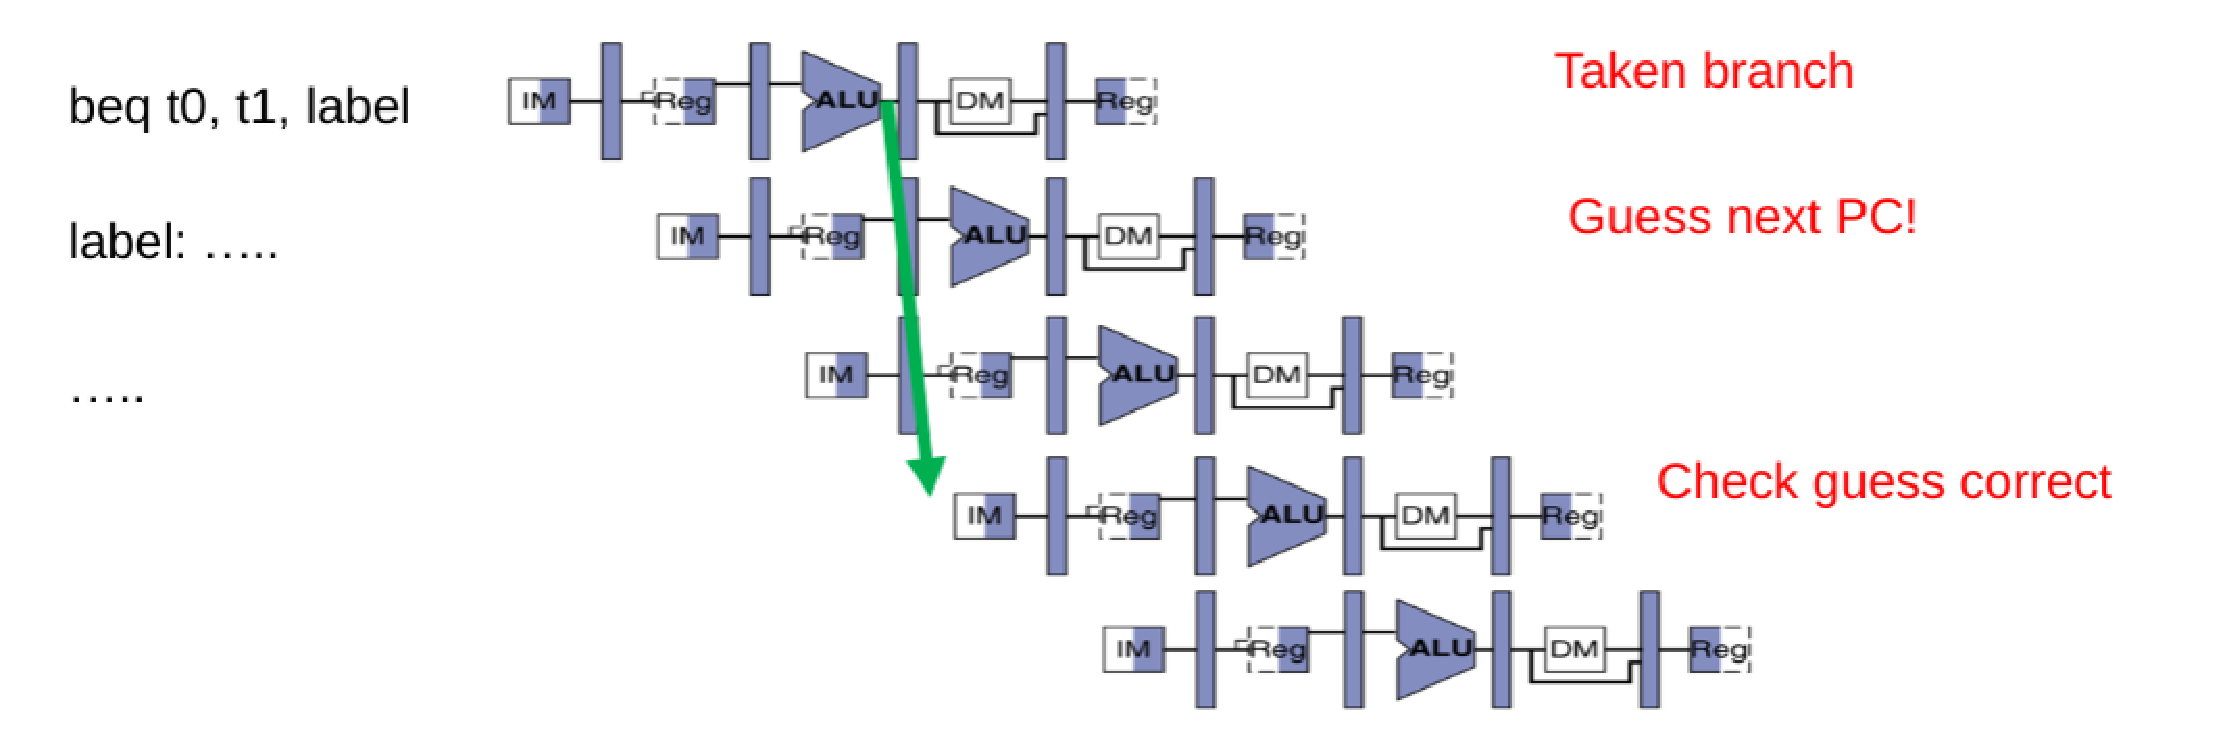
\includegraphics[width=0.8 \textwidth]{figs/RISC-V/流水线/控制冒险_预测成功.eps}
  \caption{分支预测:预测成功}
  \label{fig:Control_Hazards_Success} %设置图形引用名称
\end{figure}

\begin{figure}[htbp]
  \centering %居中显示
  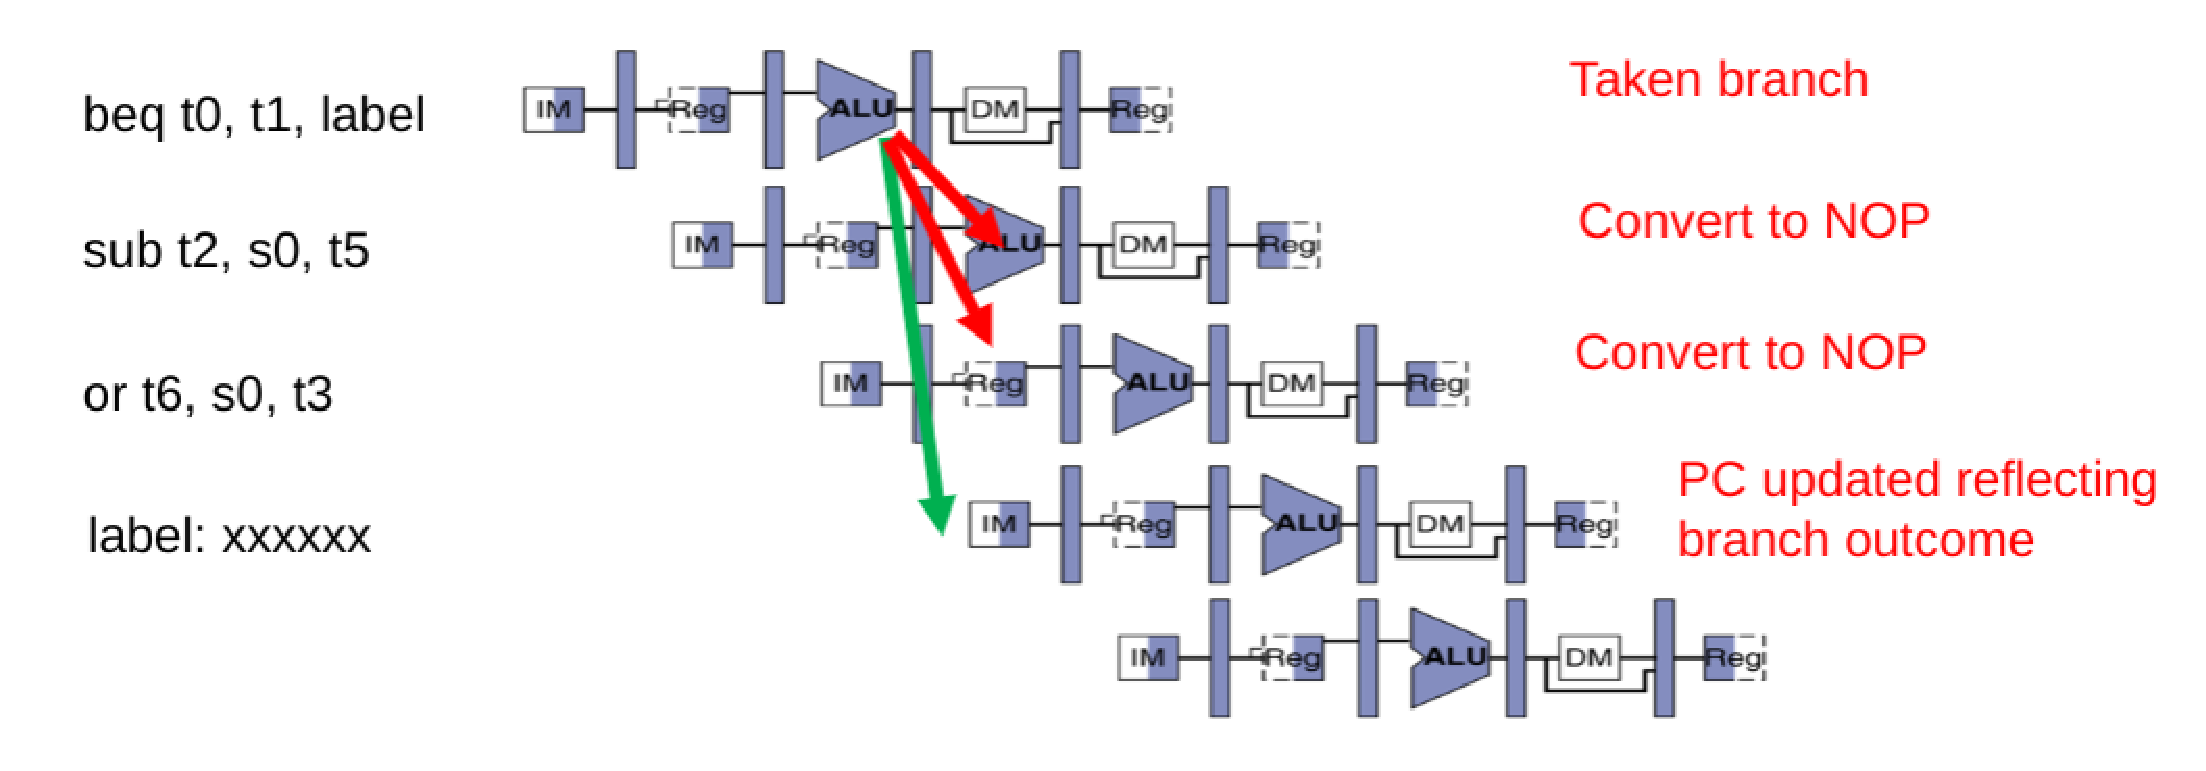
\includegraphics[width=0.8 \textwidth]{figs/RISC-V/流水线/控制冒险_预测失败.eps}
  \caption{分支预测:预测失败}
  \label{fig:Control_Hazards_Fail} %设置图形引用名称
\end{figure}







